\section{TOTAL RESPONSE}

The total response of a circuit can be teased apart into a forced response plus a natural response. These responses can be combined using the principle of superposition. This principle pressupose the addition of the natural response and the forced response, both calculated in question 3 and 4.

\subsection{Theoretical Analysis}
The final solution for $V(6)_{final}$  is then given by:
\par For t$<$0
\begin{equation}
V6_{final}=V_{6}-V_{8}
\end{equation}
\par For t$\ge$0

\begin{equation}
V(6)_{final}=V(6)_{n} + A*sin(w*t+Ph)
\end{equation}

The final solution for $V(S)_{final}$  is then given by:
\par For t$<$0
\begin{equation}
VS_{final}=Vs
\end{equation}
\par For t$ge$0

\begin{equation}
VS_{final}=1*sin(w*t)
\end{equation}

\begin{figure}[h] \centering
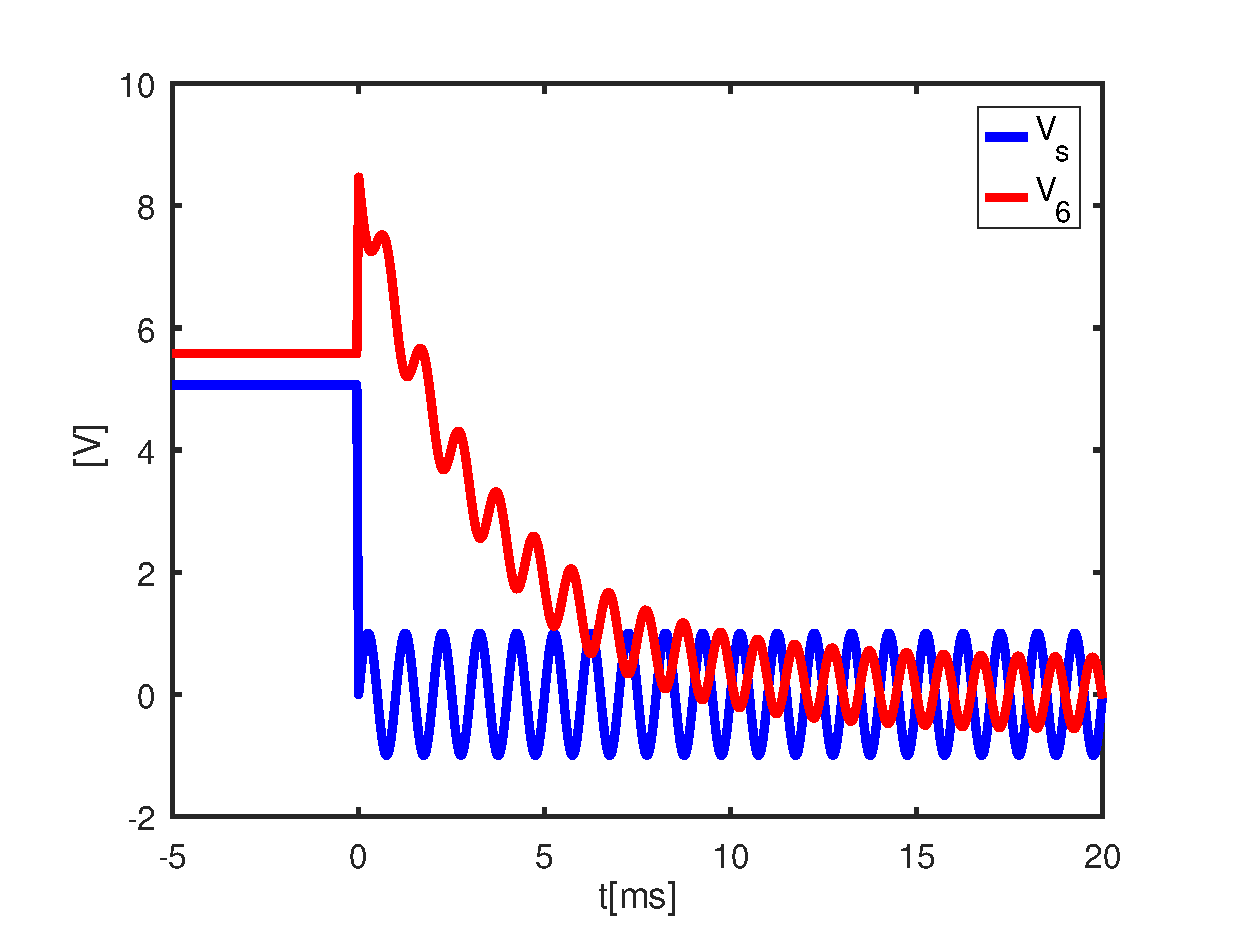
\includegraphics[width=0.5\linewidth]{part4.eps}
\caption{Circuit analysed.}
\label{fig:part4}
\end{figure}

\par It is observed in \ref{fig:part4} that $V(6)_{final}$ tends to diminuish  until 20ms, the end of the period. By this time, the phase $V(6)_{final}$ and the phase of  $VS_{final}$ differ $\pi$ or 180 degrees.


\subsection{Simulation Analysis}
Once again, a transient analysis was made in order to meet the goal above. The main difference between the analysis in question 3 and this one is that Vs was considered a sinusoidal voltage source. This way, the plot obtained is the sum of both responses.

\begin{figure}[h] \centering
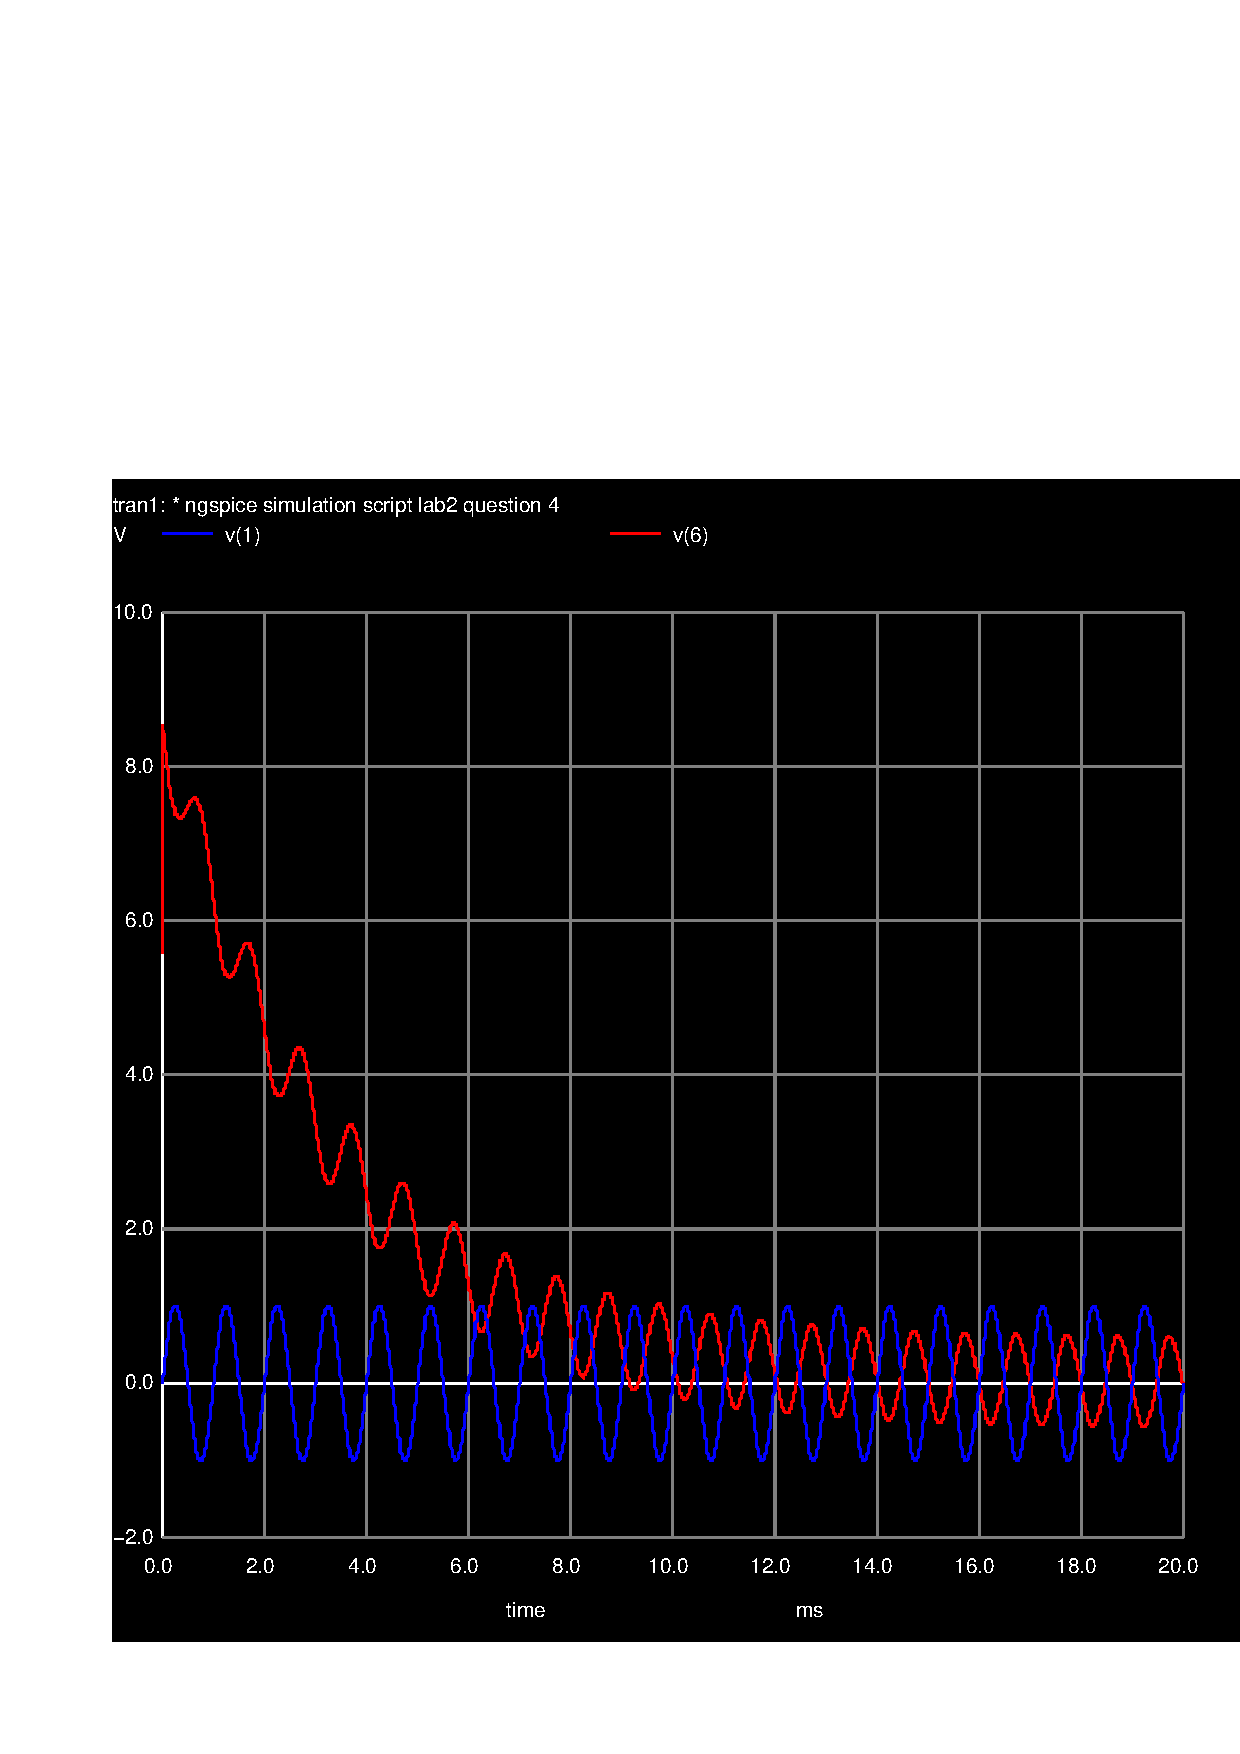
\includegraphics[width=0.4\linewidth]{sim4.pdf}
\caption{Total Response - Ngspice}
\label{fig:sim4}
\end{figure}

\subsection{Comparison}
 When observing \ref{fig:sim4}, we conclude that, in the period of time considered, the voltage in the capacitor tends to diminuish until its phase differs $\pi$ from the phase of the voltage source. The same result has also been accomplish in the theoretical analysis, as seen in \ref{fig:part4}.

\newpage
